\begin{figure}[ht!]
\centering
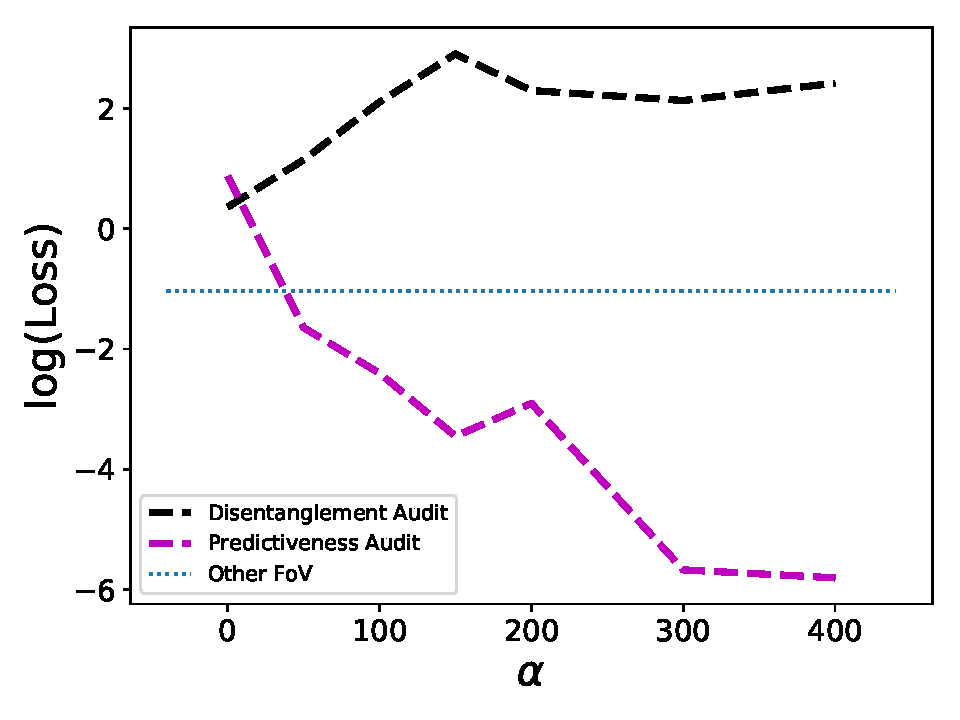
\includegraphics[width=0.4\textwidth]{dsprites_biased_val_logloss_removed_and_clf_bybetasens_a1.pdf}
\vspace{-0.2cm}
\caption{
    Black and pink dashed lines respectively show FFVAE disentanglement audit (the higher the better) and predictiveness audit (the lower the better) as a function of $\alpha$.
    These audits use $A_i$=Shape (see text for details).
    The blue line is a reference value---the log loss of a classifier that predicts $A_i$ from the other 5 DSprites factors of variation (FoV) alone, ignoring the image---representing the amount of information about $A_i$ inherent in the data.
    }
    \label{fig:dsprites-audit}
% \end{center}
% \vskip -0.2in
\end{figure}
